\documentclass[review]{elsarticle}
%%\usepackage[utf8]{inputenc}
%%\usepackage[LGR,T1]{fontenc}
%%\usepackage{graphicx,amsmath}
%%\usepackage[british]{babel}
%%\usepackage[latin9]{inputenc}%SOME KIND OF CLASH WITH THIS ONE
%%\usepackage{array}
%%\usepackage{rotfloat}
%%\usepackage{textcomp}
%%\usepackage{amssymb}
\usepackage{amsmath} 
%% to align equations \usepackage{mathrsfs} % curly font in math, called using mathscr
\usepackage{graphicx}
%%\usepackage{subcaption} % to have two images under one caption
%%\usepackage{subscript}
%%\usepackage{gensymb} %for degree symbol
\setlength{\marginparwidth}{4cm} % to set the width of the marginpar
\usepackage{todonotes}
\usepackage{makecell}
\usepackage{comment}
%%\usepackage{xargs}                      % Use more than one optional parameter in a new commands
\renewcommand{\baselinestretch}{1.5}
\bibliographystyle{elsarticle-num}
\begin{document}
\includecomment{draftversion} %change to \excludecomment{draftversion} for submission
\section{Supplementary Information}

\subsection{Stitching Method}

The individual micrographs were assembled into a composite using the 'Stitching'
plugin for Fiji/ImageJ \citep{schindelin2012fiji}, which implements the method
of Preibisch \textit{et al.} \citep{Preibisch2009}. The applied parameters are detailed in
Table \ref{tab:stitching_parameters}.

\begin{table}[hbtp]
	\centering
	\caption{Applied parameters for composite assembly applied within the Stitching plugin in Fiji}
	\label{tab:stitching_parameters}
	\begin{tabular}{l l}
		\hline
		Parameter & Setting \\
		\hline
		Stitching Type                    & Grid/Collection \\
		Type               & Filename Defined Position \\
		Overlap (\%)  & 20 \\
		Fusion Type &  Linear Blending \\
		Regression Threshold            & 0.3 \\
		Max/avg Displacement Threshold            & 2.50 \\
		Absolute Displacement Threshold            & 3.50 \\
		Subpixel Accuracy & Enabled\\
		Display Fusion & Enabled\\
		Virtual Input Images & Enabled\\
		\hline
	\end{tabular}%
\end{table}

\subsection{Variation in Automated Contrast and Brightness}

To verify the consistency of SEM parameters, metadata from the complete set of
1,350 micrographs were analysed. Contrast and brightness data extracted from the
metadata file associated with each micrograph show minimal variation across
all samples, as summarised in Table \ref{tab:contrast-brightness-summary}.

\begin{table}
	\centering
	\caption{Summary of the contrast and brightness applied by the automatic adjustment of the SEM software package for all micrographs, expressed as percentages of respective maxima for each sample.}
	\label{tab:contrast-brightness-summary}
	\resizebox{\columnwidth}{!}{%
		\begin{tabular}{lrrrr}
			\hline
			Sample & Avg. Contrast (\%) & Std. Contrast  (\%) & Avg. Brightness (\%) & Std. Brightness (\%) \\
			\hline
			IG-430B & 98.01 & 1.02 & 99.69 & 0.08 \\
			IG-430C & 98.16 & 0.82 & 99.83 & 0.08 \\
			IG-430F & 97.70 & 0.81 & 99.58 & 0.14 \\
			IG-110B & 95.86 & 0.72 & 99.26 & 0.13 \\
			IG-110C & 94.03 & 0.93 & 99.38 & 0.13 \\
			IG-110F & 98.20 & 0.70 & 99.69 & 0.13 \\
			\hline
		\end{tabular}
	}
\end{table}

\subsection{Pore Diameter Thresholding Sensitivity Analysis}
\begin{draftversion}
	\textit{\textbf{Check figure reference to main document.  
			Fig 1 caption starts: '(a). Fully assembled SEM composite.'
			Fig 3 caption starts: 'Visualisation of the effect of an increasing minimum area}}
\end{draftversion}
A sensitivity analysis, in conjunction with visual analysis, as per Figure
3 in the main document, was conducted to establish a justifiable lower
limit for pore segmentation. Based on the data in Table
\ref{tab:thresholdsandvariationsIG430F} and visual inspection of the resulting
segmentation exemplified in main document Figure 3, an area
threshold of 2 µm² was selected. This value was determined to be the optimal
compromise for excluding surface rugosity and retaining genuine porosity.

\begin{table}
	\centering
	\caption{Effect of different pore area thresholds on a subsection of IG-430 Sample F, showing the resulting pore count, total area, average pore size, and percentage area.}
	\label{tab:thresholdsandvariationsIG430F}
	\resizebox{\columnwidth}{!}{%
		\begin{tabular}{l c c c c c c}
			\hline
			\textbf{Area Threshold} (µm²) & 0 & 0.5 & 1 & 2 & 4 & 8 \\
			\hline
			Count & 254261 & 11375 & 6485 & 4085 & 2812 & 1881 \\
			Total Area (µm²) & 71219 & 56722 & 53361 & 50063.63 & 46518 & 41161\\
			Average Size (µm²) & 0.28 & 4.987 & 8.229 & 12.255 & 16.543 & 21.883 \\
			\% Area & 4.786 & 3.812 & 3.586 & 3.364 & 3.126 & 2.766 \\
			\hline
		\end{tabular}%
	}
\end{table}

\subsection{Attempted Automatic Global Intensity Thresholding}

None of the 17 automatic global intensity thresholding algorithms available in
ImageJ were able to distinguish between porosity and bulk in this dataset, as shown in Figure ~\ref{fig:Try All Thresholding Methods} below. For each sample, the histogram
\(H(i)\) produced by this method exhibited only a single peak, yielding no
statistically distinct intensity classes,  (main document, Figure 1).
This is attributed to the small area fraction represented by porosity at the
operational magnification and resolution. This low fraction fails to yield a
secondary peak for the pore phase in the histogram. These algorithms operate by
identifying a threshold value between peaks and are therefore not functional for
this dataset.


\begin{figure}[!htbp]
	\centering
	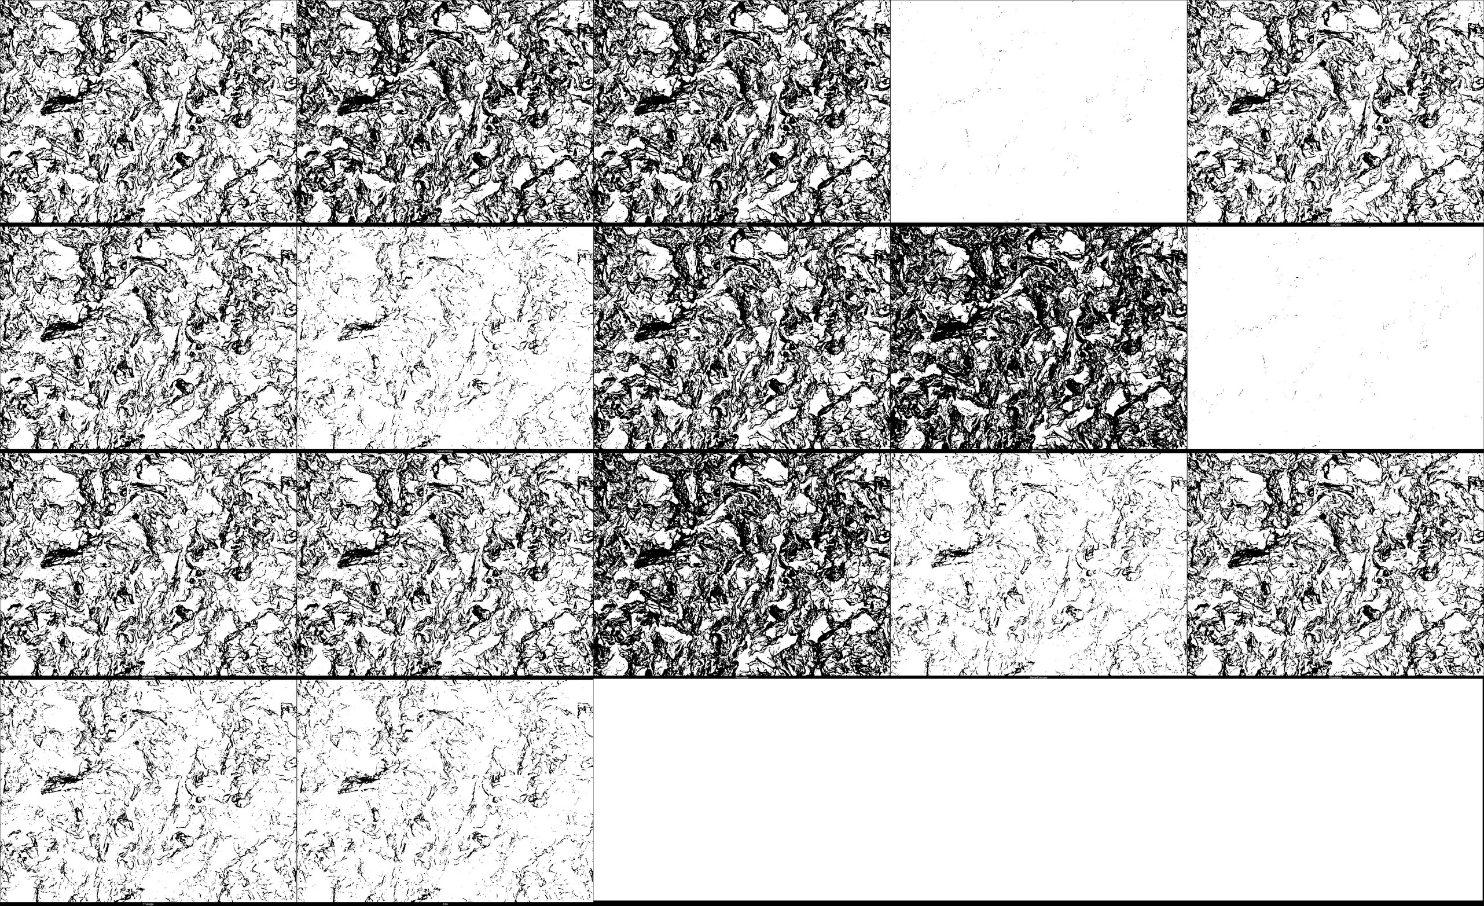
\includegraphics[width=0.9\columnwidth]{./Media/MontageIG430C MethodsNEW.png}
	\caption{Thresholded Micrograph of IG-430 Sample C at $1000\times$ Magnification. Methods placed sequentially from left to right.
		Top row:
		(a) Default
		(b) Huang
		(c) Huang2
		(d) Intermodes
		(e) IsoData.
		Second Row:
		(f) Li
		(g) MaxEntropy
		(h) Mean
		(i) MinError(I)
		(j) Minimum.
		Third Row
		(k) Moments
		(l) Otsu
		(m) Percentile
		(n) RenyiEntropy
		(o) Shanbhag
		Final Row.
		(p) Triangle
		(q) Yen}
	\label{fig:Try All Thresholding Methods}
\end{figure}  


\subsection{Modelling Sensitivity Analysis}

Sensitivity analysis consisted of assembling the five simplex parameters,
distance between simulated and experimental percolation curves, and open
porosity estimate into a single column per stochastic generation. Conditional
formatting was applied to highlight those parameters within one standard
deviation of the mean, with the stochastic generation with the lowest
distance, closest open porosity to that measured by He pycnometry for that
grade, and within one standard deviation of the mean, selected as the
representative model.
\clearpage

\bibliography{bibliography}

\end{document}
